\chapter{Entwurf}
\label{ch:3}

\section{Grobentwurf: Subsysteme}
\label{sec:3.1}
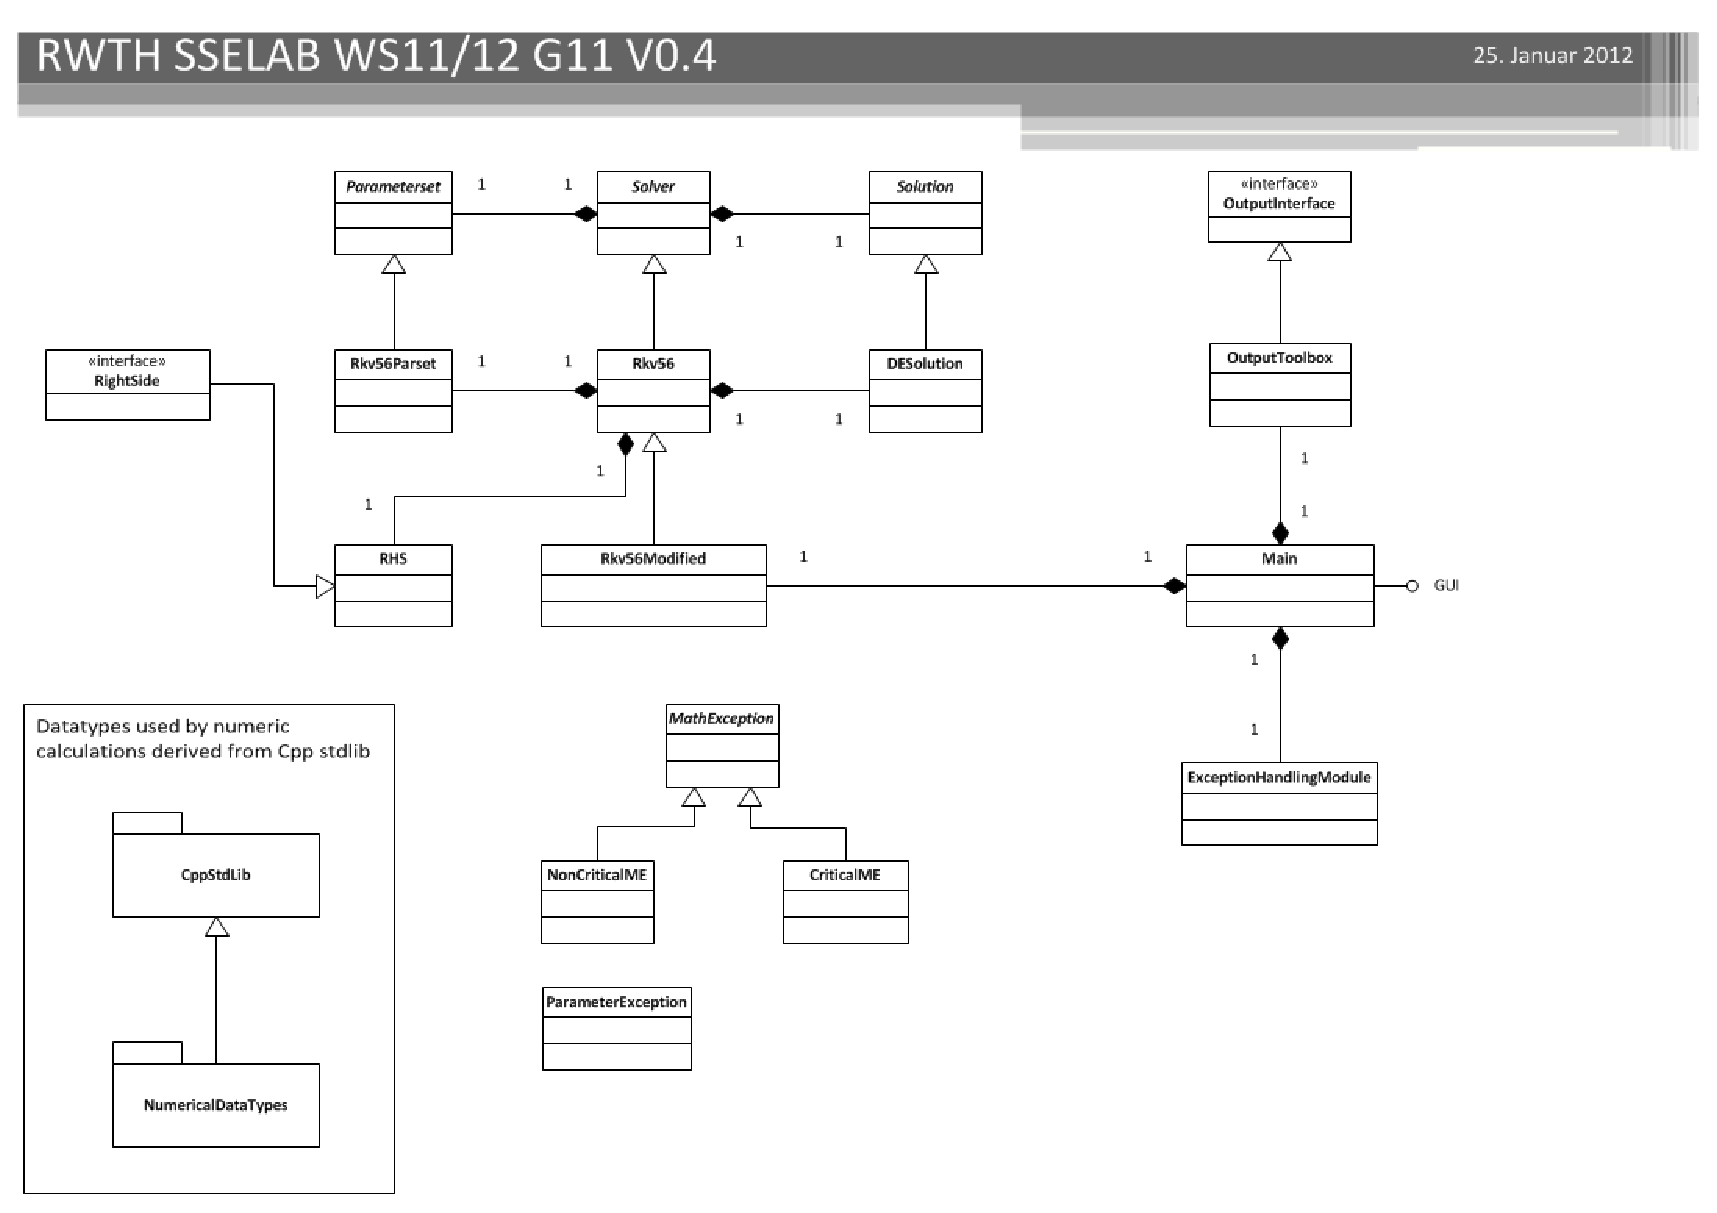
\includegraphics[width=6in,keepaspectratio=true]{figures/RWTH_SSELAB_WS1112_CLASSES.eps}

\subsection{Statik}

\subsection{Dynamik}

\section{Detailentwurf: Klassen}
\label{sec:3.2}
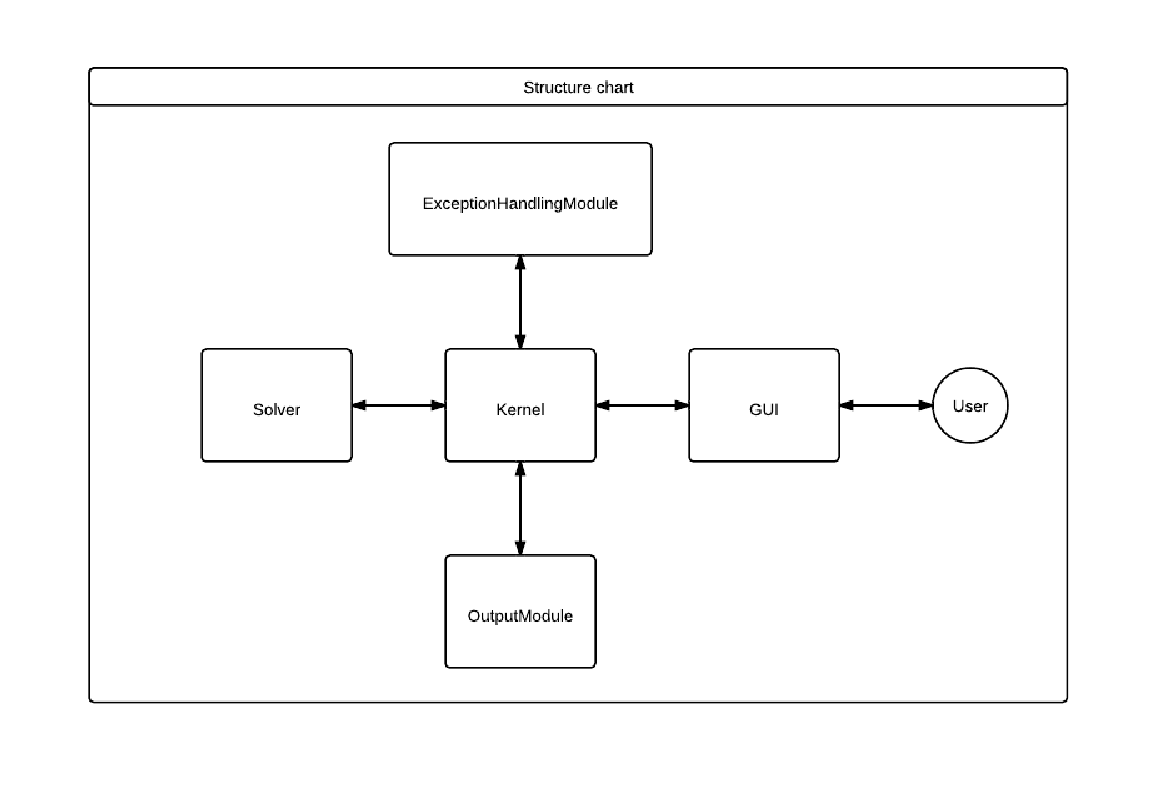
\includegraphics[width=6in,keepaspectratio=true]{figures/StructureDiagGyroSim.eps}

%%{\em Klassenmodell (Statik: Klassendiagramm; Dynamik: Sequenzdiagramm, 
%%CRC Karten) inklusive (Klassen- bzw. Objekt-)Daten und 
%%(Klassen- bzw. Objekt-)Funktionen; Navigierbarkeit; Zugriffsrechte;
%%Abstrakte Datentypen:
%%vollst\"andig spezifizierte fundamentale Datentypen, z.B. {\tt vektor}, 
%%{\tt matrix}; Axiome, Bedingungen, Testfunktionen}
%%\\
%%\\
%%\begin{itemize}
%%\item Parser basierend auf {\tt flex}\footnote{\tt http://www.gnu.org/software/flex/manual/} und
%%{\tt bison}\footnote{\tt http://www.gnu.org/software/bison/manual/}
%%\cite{Aho1986CPT,Muchnick1997ACD} zur Eingabe der Daten (Problemspezifikation)
%%\item Newton's Methode zur L\"osung des nichtlinearen Systems \cite{Kelley2003SNE}
%%\item Direkte \cite{Golub1989MC} bzw. indirekte Verfahren \cite{Saad1986Agm}
%%zur L\"osung des linearen Systems
%%\item Automatisches Differenzieren \cite{Griewank2000EDP,Wengert1964ASA} zur 
%%Berechnung der Jacobimatrix bzw. des Produkts der Jacobimatrix mit einem Vektor
%%\end{itemize}

\subsection{Statik}

\subsection{Dynamik}
\section{Graphical User Interface}
\label{sec:3.3}
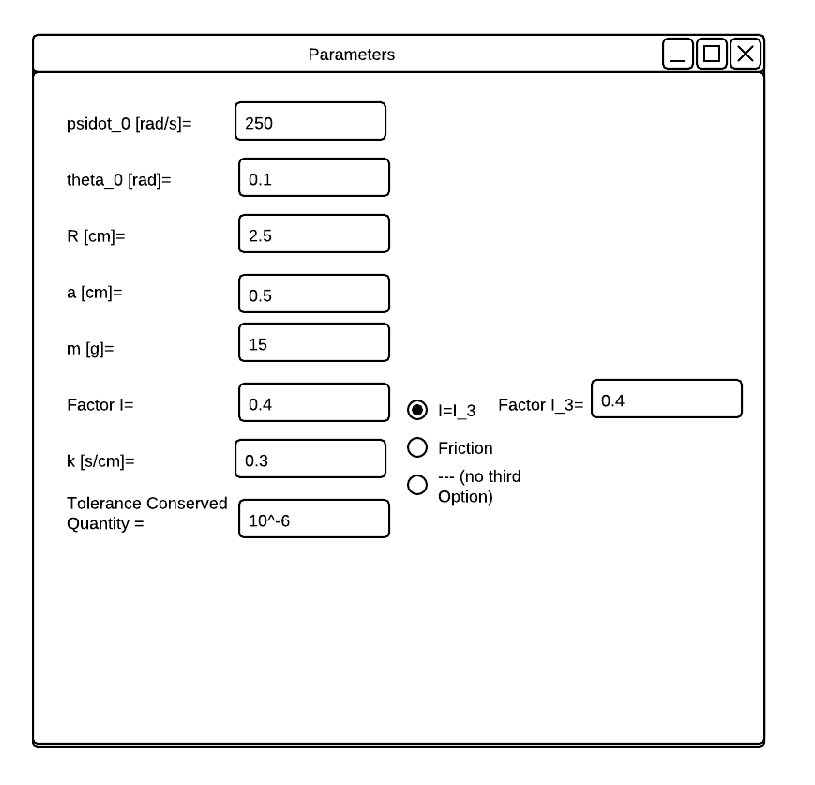
\includegraphics[width=6in,keepaspectratio=true]{figures/GUIParameterInputForm.eps}
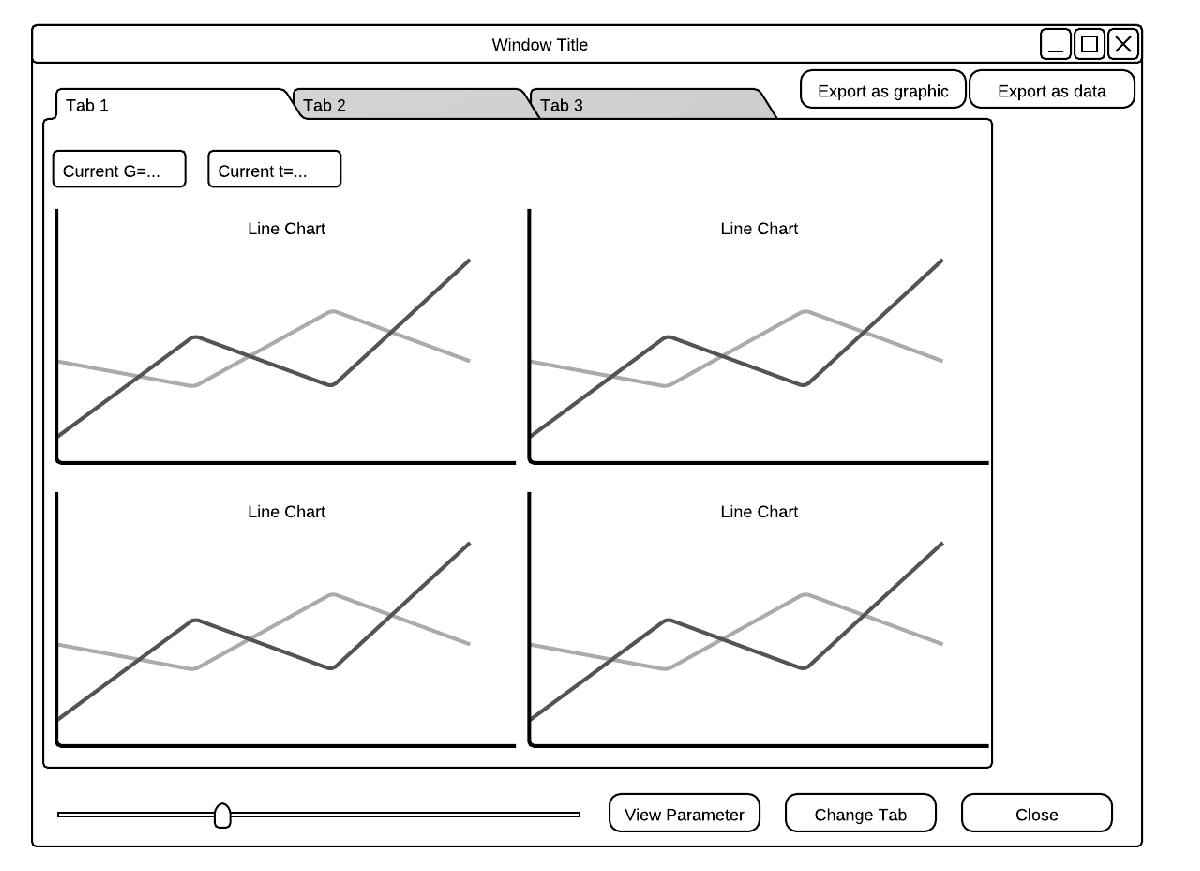
\includegraphics[width=6in,keepaspectratio=true]{figures/GUIDisplayForm.eps}
\section{Use-Case-Diagramm}
\label{sec:3.4}
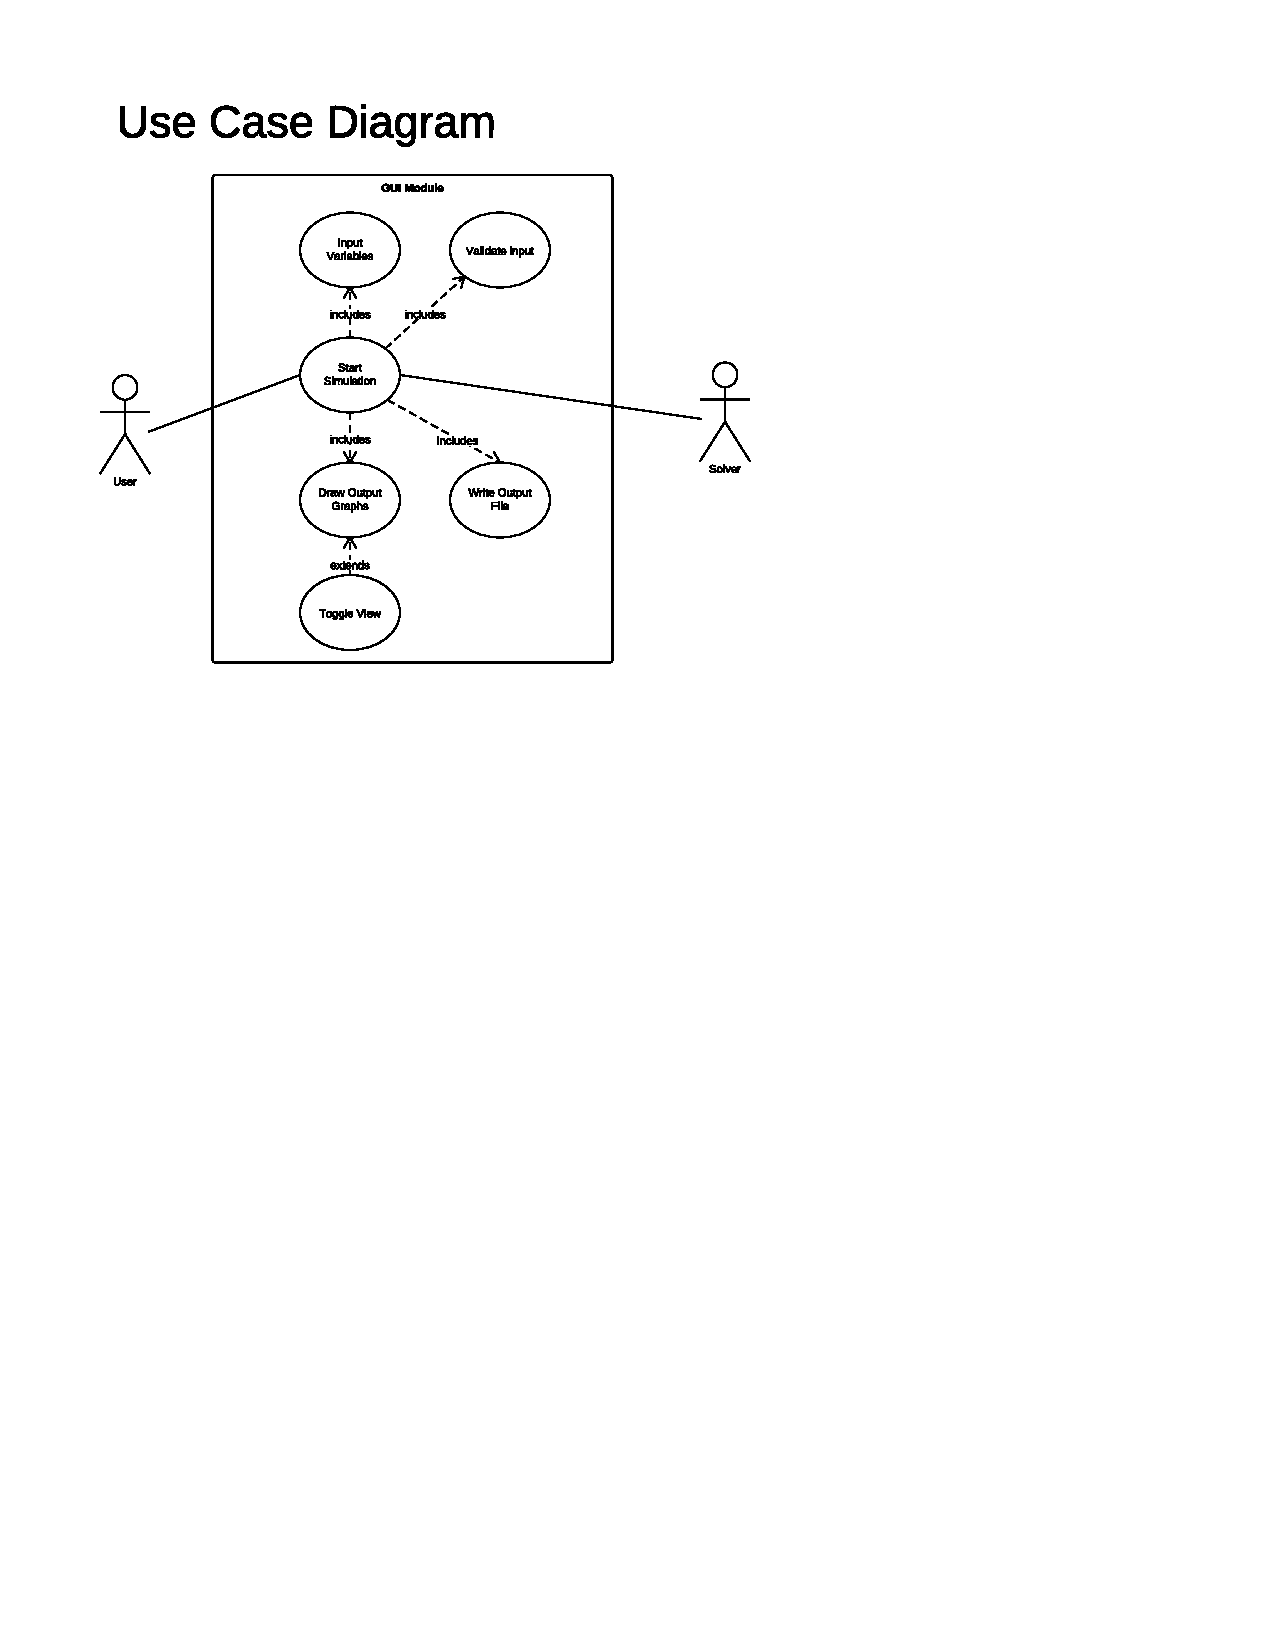
\includepdf[pages=1]{figures/UseCaseTippeTop.pdf}

